\documentclass[a4paper,twocolumn]{article}
%\usepackage{amsfonts}
\usepackage{amsmath}
%\usepackage{amsthm}
\usepackage[utf8]{inputenc}
%\usepackage{hyperref}
%\usepackage{booktabs}
\usepackage{indentfirst}
\usepackage{graphicx}
\usepackage{subfig}

\graphicspath{{fig/}}

\title{Fun with Pong}
\author{Cédric Bhihe and Rodrigo Arias}
\date{\today}

% Useful vectorial and matrix notation
\newcommand*\mat[1]{ \begin{pmatrix} #1 \end{pmatrix}}
\newcommand*\arr[1]{ \begin{bmatrix} #1 \end{bmatrix}}
\newcommand*\V[1]{ \boldsymbol{#1}}

\begin{document}
\maketitle

% What it is asked to write here:
%
% It is expected that you make a proposal for the project for preliminary
% evaluation. Proposals should be submitted through the racó no later than April
% 9th, 2018. Submit your proposal as a 1-page pdf; it is enough that one member
% of the team submits this through the racó. Your project proposal should
% specify which problem you want to tackle, why you choose this problem, a
% couple of fundamental references, a preliminary title, and a list of team
% members.
%
% NOTE: They don't ask HOW to solve the problem. 

\section*{Introduction} % Background introduction to Pong

Pong is one of the earliest video games, released in 1972 by Atari. Is a
2-players table tenis sport game built with very simple 2D graphics.

% [Pong image]
\begin{figure}[h]
	\centering
	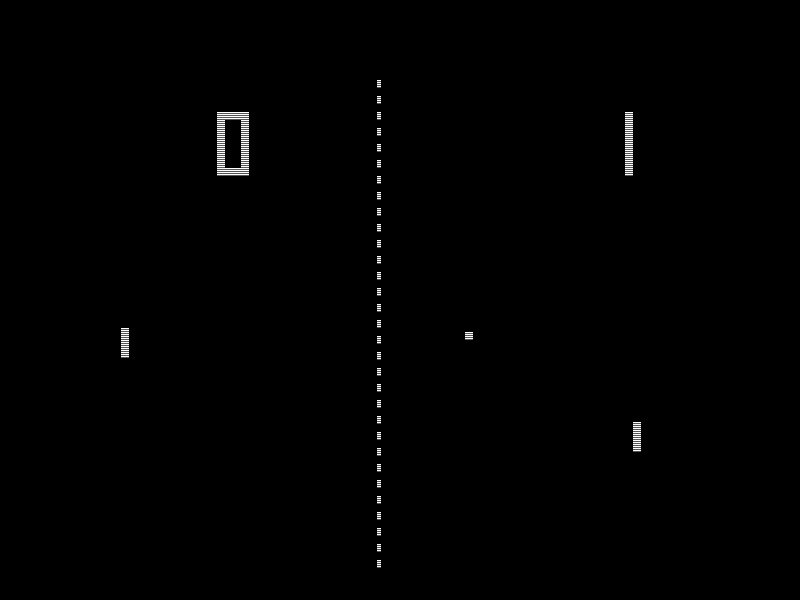
\includegraphics[width=0.7\columnwidth]{pong.png}
	\caption{Original Pong game}
	\label{fig:pong}
\end{figure}

Each player controls a paddle by moving it vertically across the table, in order
to hit the ball. The objective of the game is to make the opponent miss the
ball. Each ball missed scores a point to the opponent, and a new exchange
starts. The ball can bounce off the paddles as well as the side walls.

\section*{Proposal} % Description of the problem, NOT the solution

We propose the design and implementation of player controller agents by using 
different machine learning methods. The agent should be able to move the paddle 
as a human would do.  The objective of the project is to compare the performance 
of various ML agents against one another. In order to test them a tournament is 
played, such that the winners will play against each other until there is only 
one winner.

Given the nature of the problem we choose to focus on reinforcement methods like 
Q-Learning~\cite{SuttonBarto98}. Different agents can be either complete 
different RL methods or only with small differences in the parameters.

We may introduce incremental complexity in the successive games so as to make
learning by the ML agents gradually more difficult. Some examples may include:

% This are only examples, we don't need to stick to those

\begin{itemize}
	\item Paddles with mass to constraint the moves.
	\item Holes in the space covered by the paddles, which a trained player could
		exploit.
	\item Non-uniform bounces in the paddles to modify the trajectory of the ball.
\end{itemize}

% XXX: We don't know this yet! This is part of the actual implementation.
%
% Their actions is (UP, DOWN, STAY), or in a more sophisticated modality
% (UP-SLOW, UP-FAST, DOWN-SLOW, DOWN-FAST, STAY).  Those methods are introduced
% later in this proposal and are meant to help define the project’s scope in a
% qualitative way.

\section*{Motivation} % Why we choose this?

One of the main reasons to choose a game like the Pong, is the simplicity. We
can focus on different methods, so we can learn without spending a lot of effort
in the implementation. The game is very common and likely to be already
implemented, so we can reuse parts of it.

As we control the problem, we can adjust the complexity of the game as far as we
want. So we are not fixed by a complex problem, but a simple one that we---as
humans players---already know how to solve. Reinforcement methods can deal with 
incomplete knowledge problems, which are very common in the real life. Once we 
understand how to apply them to a simple problem, we can continue to more 
complex problems.

% References. Très important!

\bibliographystyle{siam}
\bibliography{biblio}

\end{document}
